\section{Background(Yang)}\label{sec:background}
Our approach is based on Atmel AVR Toolchain and focuses on AVR microprocessors. In this section, we discuss the necessary background knowledge related to our approach, such as AVR architecture, AVR Toolchain, etc.

%\subsection{SBU and MBU}\label{sec:sbu_mbu}
%Single Event Upset (SEU) is defined by NASA Thesaurus as "Radiation-induced errors in microelectronic circuits caused when charged particles (usually from the radiation belts or from cosmic rays) lose energy by ionizing the medium through which they pass, leaving behind a wake of electron-hole pairs."
%When high-energy ionizing particles passes through and ionize a memory cell, the bit stored in that memory cell may flip: $0 \Rightarrow 1$ or $1 \Rightarrow 0$. This occurrence is known as Single Bit Upset (SBU). It also has been observed that a single particle can flip two or more bits in adjacent memory cells. This occurrence is known as Multiple Bit Upset (MBU), which only constitutes about 3 percent in all the memory errors that occurs in space.\cite{shirvani2000software}. Thus it would be more practical for our approach to solve the SBU problems first, which takes significantly more weight in all memory errors.

\subsection{AVR Architecture}
AVR microprocessors are based on the Modified Harvard architecture~\cite{argade1996apparatus}, which stores instructions and data in physically separate memories, flash memory and SRAM, and concurrently accesses instructions and data through separate memory buses. The flash memory, which is non-volatile and with high capacity but slow access speed, is used to store executable programs composed of AVR instructions. The SRAM, which is volatile and with low capacity but fast access speed, is used to store data used by the executable programs during runtime. For example, the ATmega644 used in this paper consists of a 64KB flash memory, a 4KB SRAM, a 16-bit instruction bus and an 8-bit data bus. Below is a description of the SRAM, as well as the registers, in the AVR microprocessor used in our approach.

\subsubsection{AVR SRAM}
The address range of on-board SRAM of ATmega644 is from 0x0100 to 0x10FF, which can be extended to address 0xFFFF by using external RAM, shown in Figure \ref{fig:ram_map}. 
The AVR SRAM is partitioned into sections, each of which is used to store different types of data. The \textit{.data} section is used to store the initialized static variables and global variables. The \textit{.bss} section is used to store the uninitialized static and global variables. The size of pre-allocated SRAM is the sum of the sizes of .data and .bss sections, which are decided at compile time. The remaining space in SRAM is shared by the heap and stack sections. The \textit{heap} section is used to store dynamically allocated memory when function \textit{malloc()} is called \cite{goldt1995linux}. The \textit{stack} segment is used to store return address, actual parameters, conflict registers and local variables and other information. The \textit{stack} can be used both by the internal control from microprocessor as well as the programmer to store data temporarily. The stack operates with a Last In First Out (LIFO) mechanism, which grows downwards, towards to lower address.

\begin{comment}
\begin{enumerate}
\item[•]
\textbf{EEPROM}
EEPROM stands for Electrically Erasable Programmable Read-Only Memory. Any new data once written, will remain in the EEPROM forever until it has been electrically erased. The primary trade-off for this improved functionality is higher cost. And the write cycles are also significantly longer compared to RAM. Thus EEPROM is not the best choice for main system memory.
\item[•]
\textbf{Flash Memory}
Flash memory is also non-volatile, with high capacity but slow access speed. ATmega644 microprocessor has 64K Bytes programmable flash which is used to store the program and a bootloader, which is a special application positioned in a special region, 256 Bytes to 4 KB, in the flash memory. The feature of bootloader is at reset, the bootloader will run first and then choose to re-program or jump to the main application according to the user-programmed options. 
\item[•] 
\textbf{SRAM}
SRAM stands for Static Random-Access Memory, which is used as the main system memory to store the data processed during run time because of the high access speed. The SRAM within AVR architecture includes 32 General-Purpose Registers, 64 I/O Registers and Data Segment.
\end{enumerate}

\begin{figure*}[t]
\centering
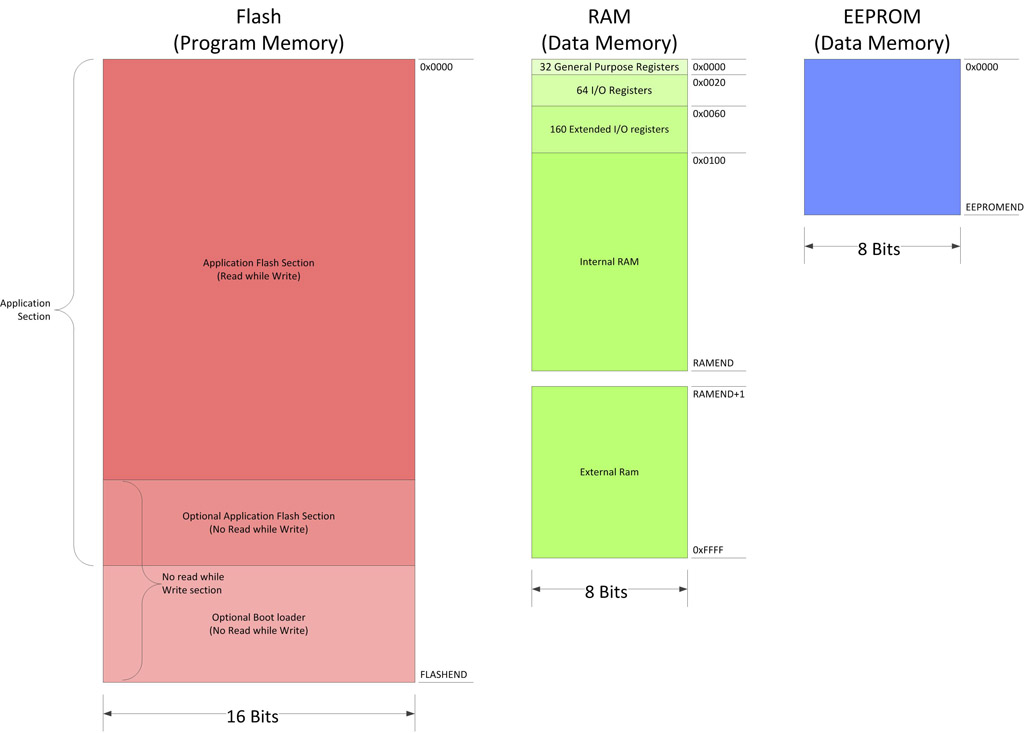
\includegraphics[width=1\textwidth, height=12cm]{figures/AVRMemMap.jpg}
\caption{AVR Memory Structure}
\label{fig:AVR_Memory_Map}
\end{figure*}

\begin{lstlisting}[float=tb,label=lst:stack_frame,caption=Assembly Code Example]
int main(void)
{
	...
	foo(arg1, arg2, ..., argM);
}

void foo(arg1, arg2, ...,argM)
{
	int var1, var2, ..., varN;
	...
}
\end{lstlisting}
\end{comment}

\begin{figure}
\centering
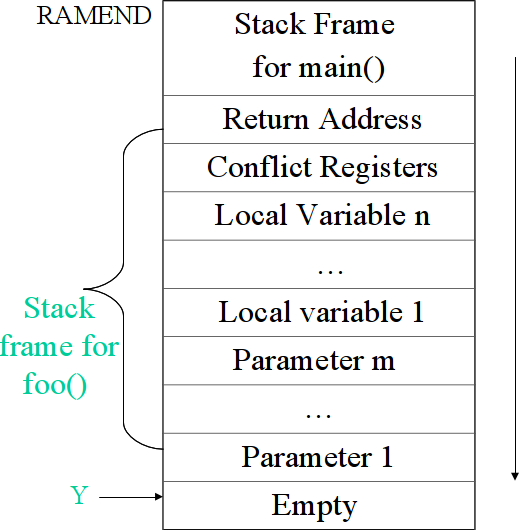
\includegraphics[scale=0.3]{figures/stack_frame.png}
\caption{AVR Stack Frame}
\label{fig:stack_frame}
\end{figure}
\subsubsection{Stack Frame}
Inside the stack are stack frames, each of which is a region in the stack used by a function. The stack frame is created when a function is called and is freed when the function returns. For example, as shown in Listing \ref{lst:stack_frame}, when function \textit{main} calls function \textit{foo}, the space allocation process for function \textit{foo} starts. First, the return address of function \textit{foo} will be pushed into the stack, followed by the conflict registers. Then the local variables, and parameters of function \textit{foo} will be pushed into stack in reversed order. After these steps, the space that the function call needed has been allocated. The stack frame of function \textit{foo}, from the return address through with first parameter, is created. The stack frame pointer will point to the next available address in the stack as well as the Stack Pointer (SP). When the function \textit{foo} finishes execution and need to return, the stack frame will be freed while the stack frame pointer and the Stack Pointer will point back the next available position after the stack frame of function \textit{main}.


\subsubsection{Registers}
%As shown in Figure xxx, the ATmega644 is equipped with 32 general purpose registers, R0 to R31, two stack pointer registers, \_\_SP\_L\_\_ and \_\_SP\_H\_\_, and a status register, \_\_SREG\_\_. The utilization of different registers is compiler-specific. The AVR-GCC used in this paper utilizes R28 and R29 as the stack frame pointer, \texttt{Y}, which points to the next available position after the stack frame of the function being processed currently.

As shown in Figure x, the General-Purpose Registers, R1 to R32, are mapped into the first 32 bytes of the SRAM, and can be directly used in assembly commands to access and store instructions in the SRAM. Some General-Purpose Registers are used as a pair for special purpose. For example, R29 and R28, the Y-Pointer, is used to indicate the Stack Frame, which will be explained in the next subsection. The operations to the different registers are compiler-specified. For example, the AVR-GCC compiler uses R24 and R25 to store the return value of a function call. Since wrong operations to the registers can bring fatal errors or high cost, it is important to limit the number of registers manipulated by our approach and manipulate them in an appropriate way.

The 64 I/O Registers, written as \textit{0x00} through \textit{0x3F}, are mapped into the next 64 bytes of the SRAM, and actually present the address section from \textit{0x20} to \textit{0x5F} in the SRAM,  shown in Figure \ref{fig:IO_REG}. Some I/O Registers are used as a pair for special purpose. For example, \textit{0x3E} and \textit{0x3D}, are used as the Stack Pointer (SP), which indicates the current top of the stack.


\begin{figure}
\centering
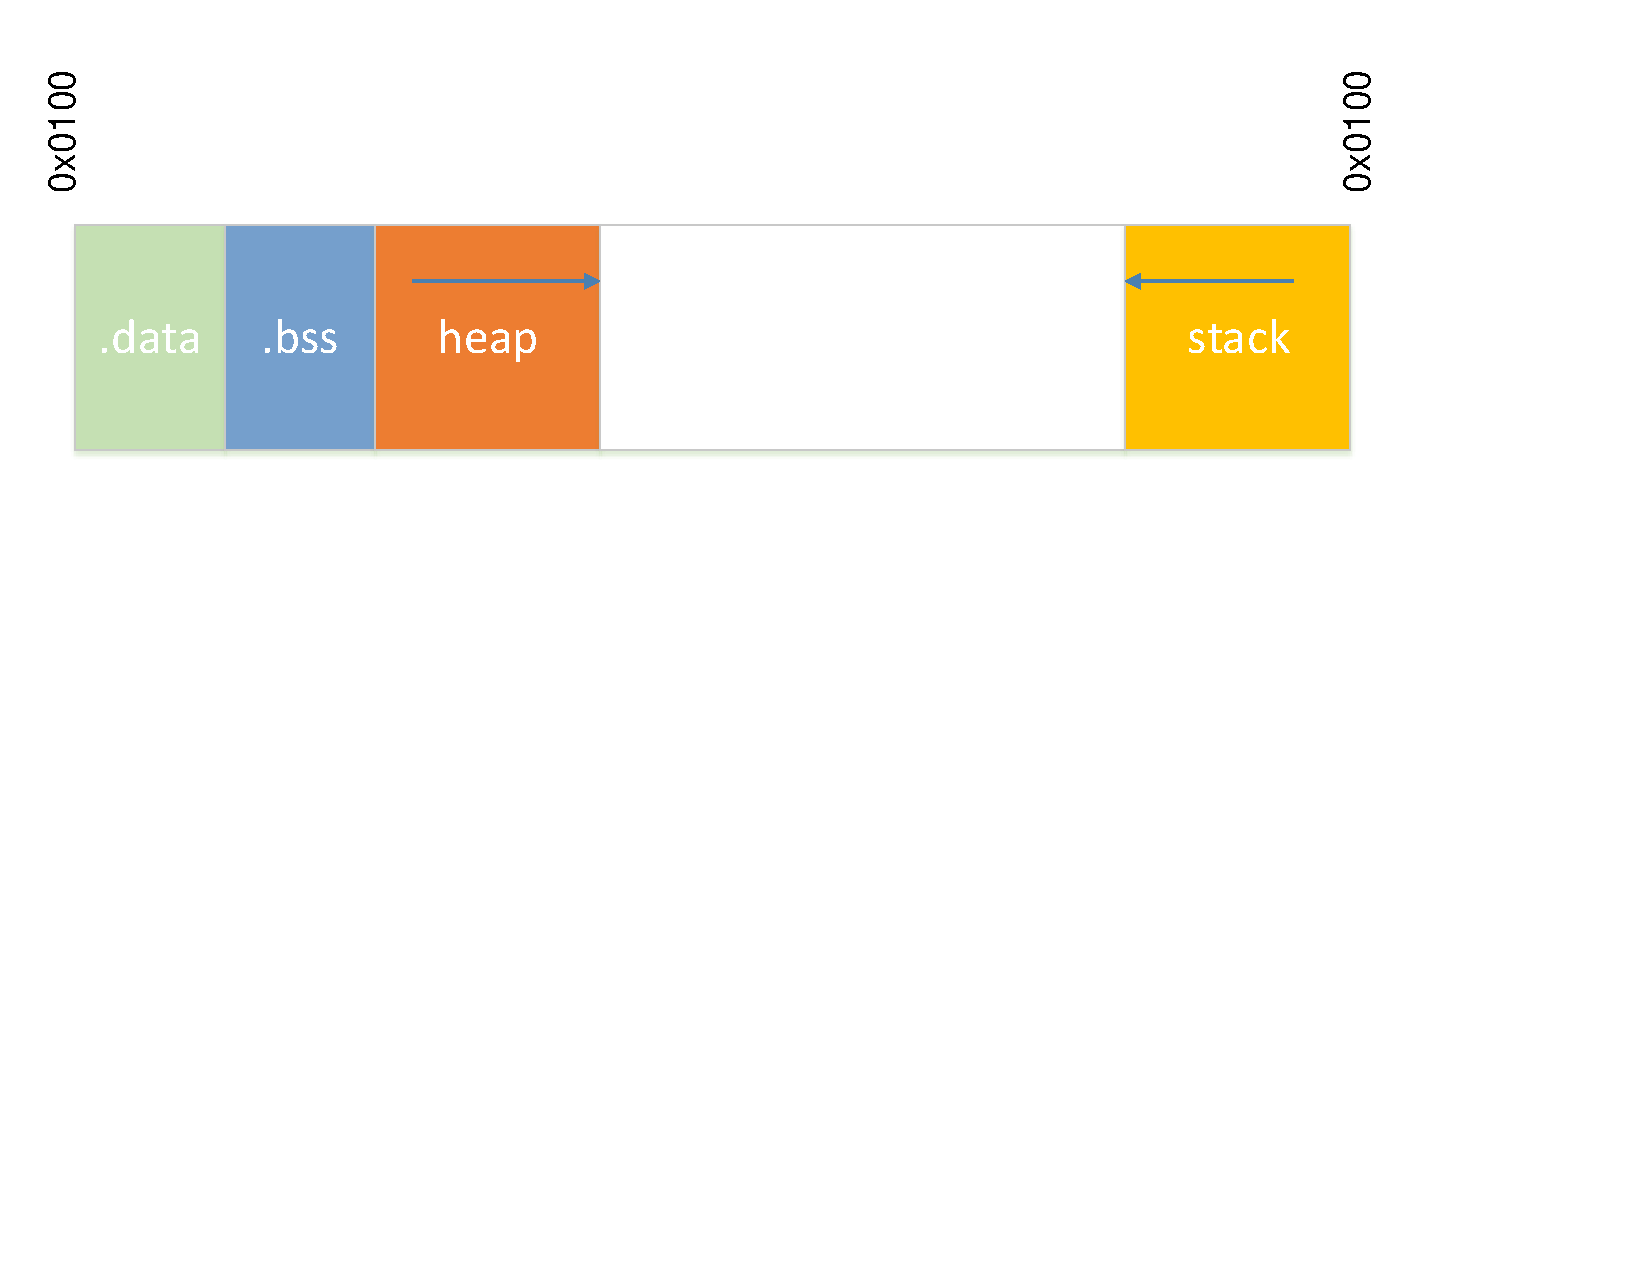
\includegraphics[width=0.5\textwidth]{figures/Memory_model.pdf}
\caption{AVR RAM Map}
\label{fig:ram_map}
\end{figure}




\subsection{Function Call Process}

Function calls follow the same process, and use the system stack to perform most operations, demonstrated in Figure \ref{fig:original_function_operation}. Figure \ref{fig:original_function_operation_process} shows the execution process when a function is called, with each operation labeled with a number. Figure \ref{fig:original_function_operation_stack} shows the system stack changes after each operation is performed. The numbers below each stack show the operations that change the stack. \texttt{SP} is the stack pointer, and \texttt{Y} is the stack frame pointer. When a function is called, the return address is automatically pushed into the stack by one of the function call instructions, \texttt{call}, \texttt{rcall} and \texttt{icall} (step 1. 1 is the operation number, similarly hereinafter). After the stack frame pointer is pushed (step 2), the stack frame of the function is created by change the stack pointer and stack frame pointer (step 3). The arguments and local variables are then pushed into the stack (step 4), and the function starts to execute (step 5). The arguments and local variables are released after the function finishes its execution (step 6), and the stack frame pointer is restored (step 7). Finally, the function returns (step 8). The return address is popped and used when one of the function return instructions, \texttt{ret} and \texttt{reti}, is called.



\begin{figure}
        \centering
        \begin{subfigure}[b]{0.5\columnwidth}
                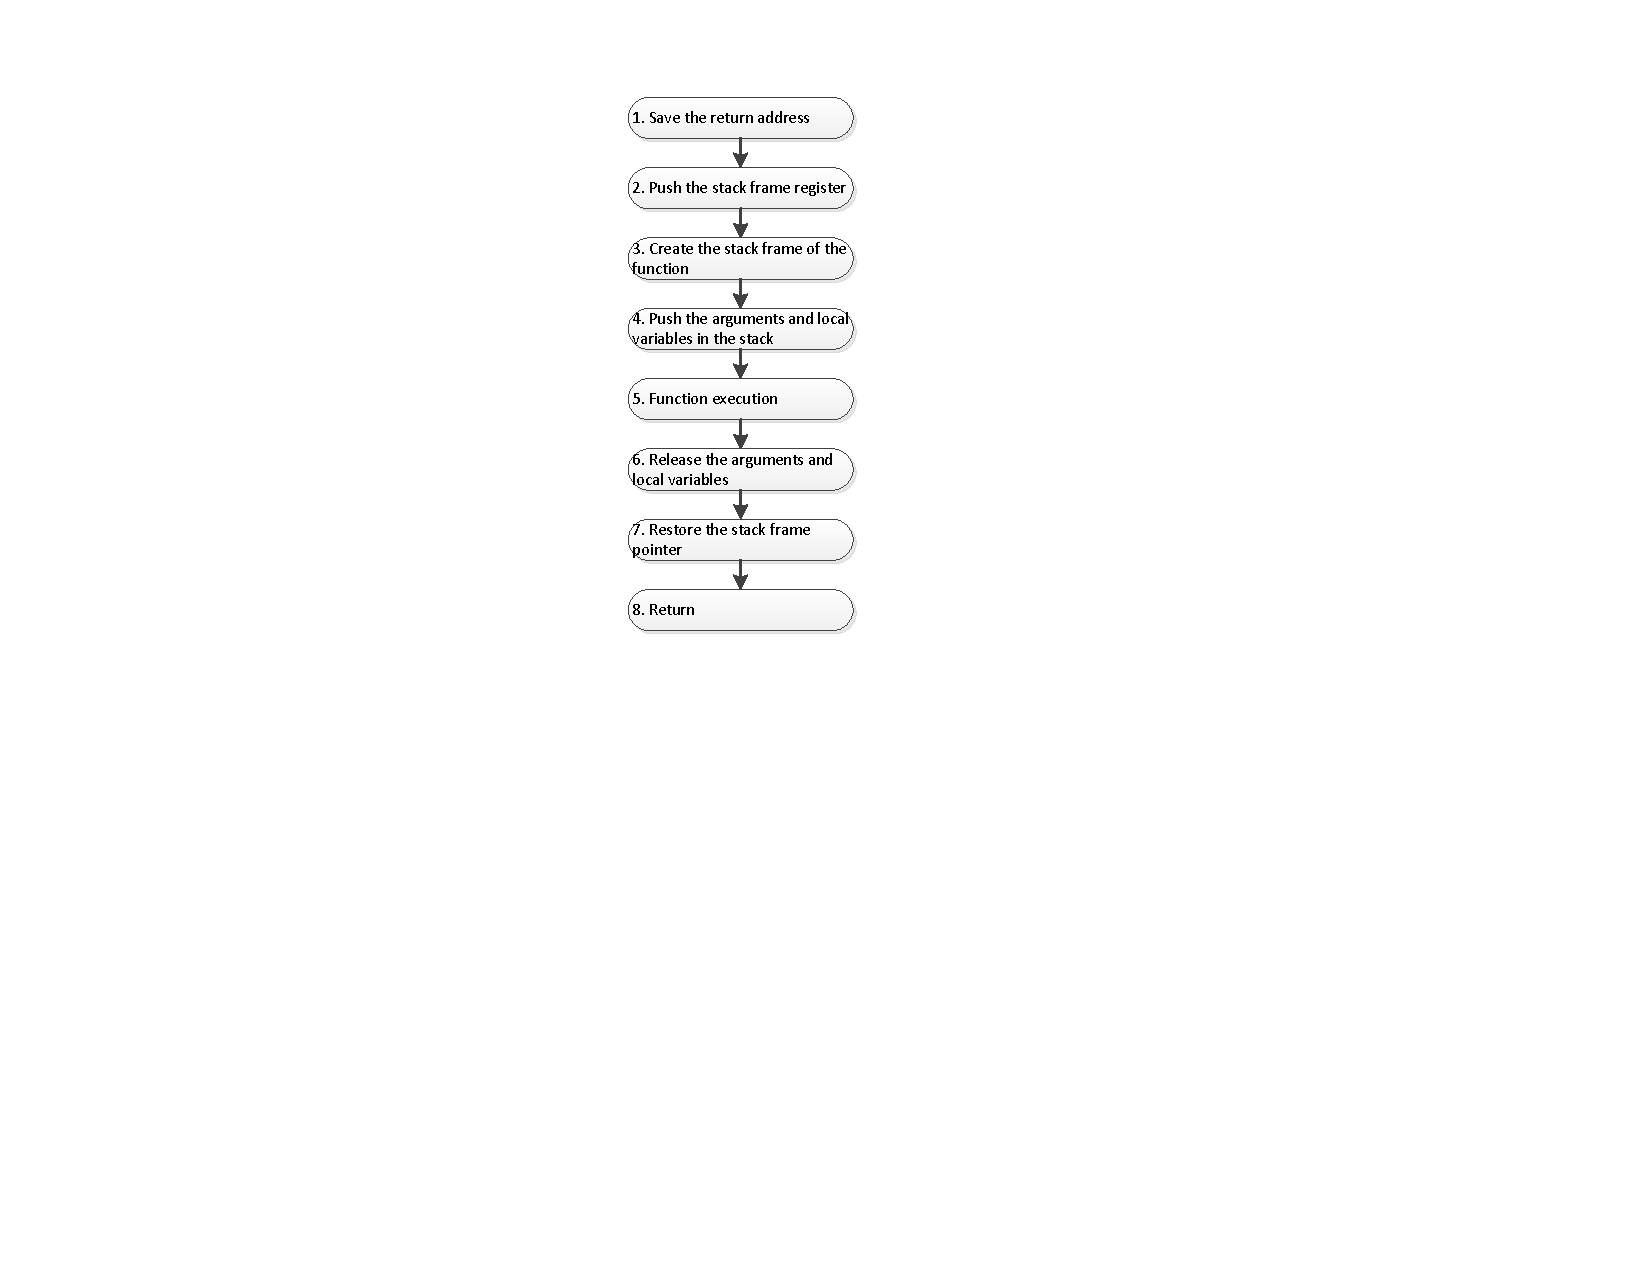
\includegraphics[width=\textwidth, height=12cm]{figures/original_function_operations_process_v1}
                \caption{Process}
                \label{fig:original_function_operation_process}
        \end{subfigure}~
        \begin{subfigure}[b]{0.5\columnwidth}
                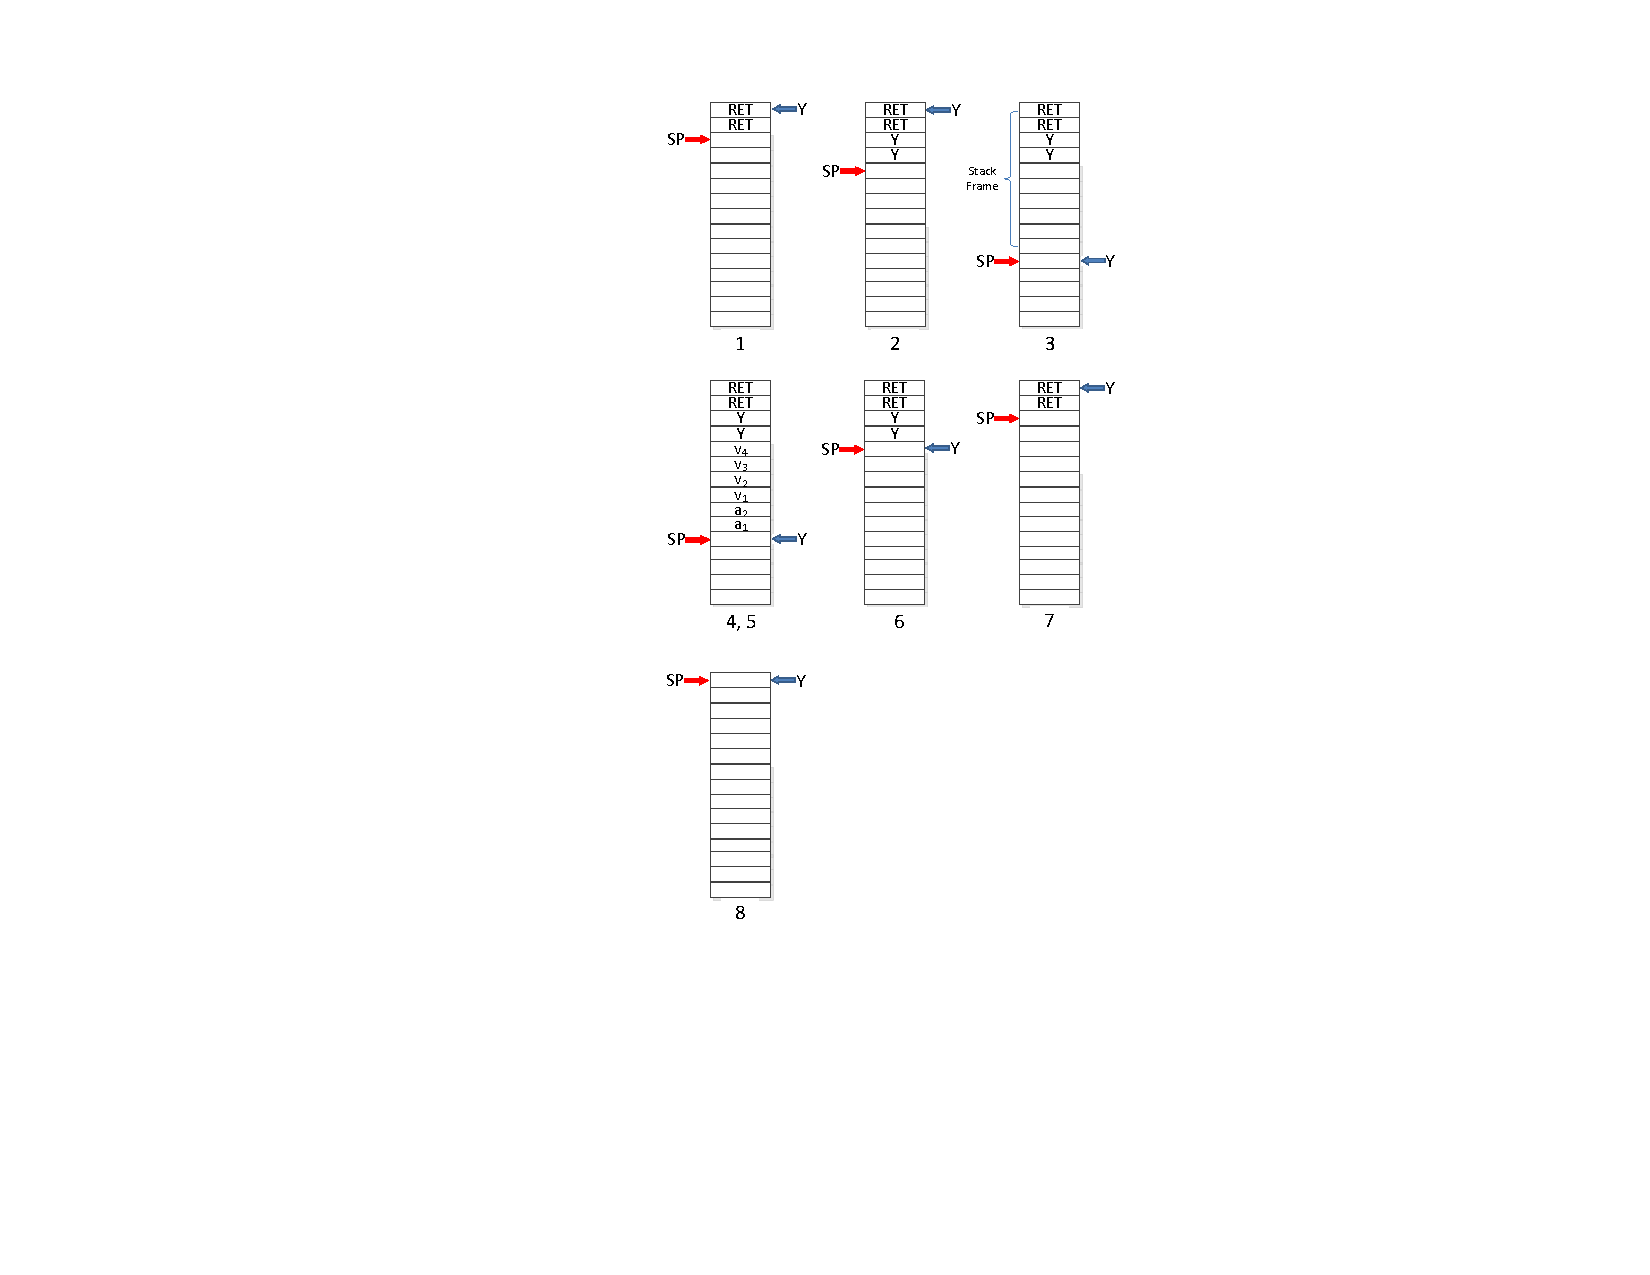
\includegraphics[width=\textwidth, height=12cm]{figures/original_function_operations_stack_v1}
                \caption{Stack}
                \label{fig:original_function_operation_stack}
        \end{subfigure}
        \caption{Function execution}\label{fig:original_function_operation}
\end{figure}

\subsection{Atmel AVR Toolchain}
Atmel AVR Toolchain is a collection of tools used to generate executable programs for AVR microprocessors. The AVR Toolchain consists of the following tools.

\begin{itemize}

\item \textit{avr-gcc}, an extension of the GNU GCC, is a cross compiler which translates a high-level language, e.g., C and C++, to assembly code for the AVR microprocessors.

\item \textit{avr-as} is the assembler which translates the assembly program to object file for the AVR microprocessors.

\item \textit{avr-ld} is the linker which uses the Linker Script to combine object modules into an executable image suitable for loading into memory of the AVR microprocessors. By using customized Linker Script, the default memory structure of the AVR microprocessor can be changed and new data structures can be added.

\item \textit{avr-libc} is a standard C library which contains many standard C routines as well as many additional AVR-specific library function.

\end{itemize}

As a matter of convenience, the AVR Toolchain could be used to compile, assemble, and link C program in one command. But to modify the code of the AVR applications in assembly-level and use customized Linker Script, these steps need to be done individually.


When the avr-gcc compiler is used to compile the source code, C program, to assembly program, there are 5 controllable optimization levels \cite{hoste2008cole}. We implement our approach at level \textbf{O0}, which is without optimization. since the generated assembly code will show the original behavior of the source program without optimization, the operations to stack can be displayed more obviously. Meanwhile, it would be more convenient for developing, debugging, and evaluating. 